\chapter{Background}
\label{cha:background}

%This chapter briefly covers the binary search algorithm, the background of Gaussian Processes, and relevant studies using Gaussian Processes. 
This chapter briefly covers related work done using spatio-temporal datasets, the background of Gaussian Processes and relevant studies using Gaussian Processes. 
Various evaluation metrics are explained, alongside the GPflow framework used for the Gaussian Process model implementations.
Finite-state machines are defined and various techniques in the area of Exploratory Data Analysis are explained. 

\section{Related Work With Spatio-Temporal Datasets}
Datasets similar to the one explored in this thesis project have been used in recent studies.
For example, in \cite{JIT1699}, trajectory datasets are used to model latent driving patterns and qualitatively analyse the main intentions of travelling drivers.
The model can be used to learn the preferences of individual drivers and to understand the context in which the driver travelled.
Crowdsources bus data is used in \cite{Kong2018} to explore traffic problems by using an anomaly detection method.
In \cite{DABIRI2018360}, a dataset of trajectories is used to create a model of transportation modes for users.
Transportation agencies can use the model to analyse the mode of transportation and identify regions where the transit systems can be improved. 


% \section{Binary Search}
% Binary search is a common algorithm for searching through a sequence for a target value.
% The algorithm utilises a binary tree for the search.
% The algorithm can be described by the following steps, from Knuth \cite{Knuth1971}:
% \begin{enumerate}
%     \item If the tree has no root node, the search is unsuccessful. 
%     The target value is not in the tree, as the tree is empty.
%     \item If the root node has the target value, the search is successful.
%     The position of the target value is found.
%     \item If the target value is smaller than the root value, the left side of the binary tree is explored.
%     The algorithm returns to the first step of the procedure.
%     This time the tree is the left half of the binary tree, with the new root node being the left child of the previous root node.
%     \item If the target value is greater than the root value, the right side of the binary tree is explored.
%     The algorithm returns to the first step, but this time the tree is the right subtree of the binary tree.
%     The new root node is the right child of the previous root node.
% \end{enumerate}
% The procedure is illustrated in Figure \ref{fig:binary-search-algorithm}.
% The algorithm has a complexity of $O(log_2 n)$, as the search space is in the binary case divided in two after each comparison.
% However, the algorithm requires a sorted sequence of values.

% \begin{figure}[t!]
%     \centering
%     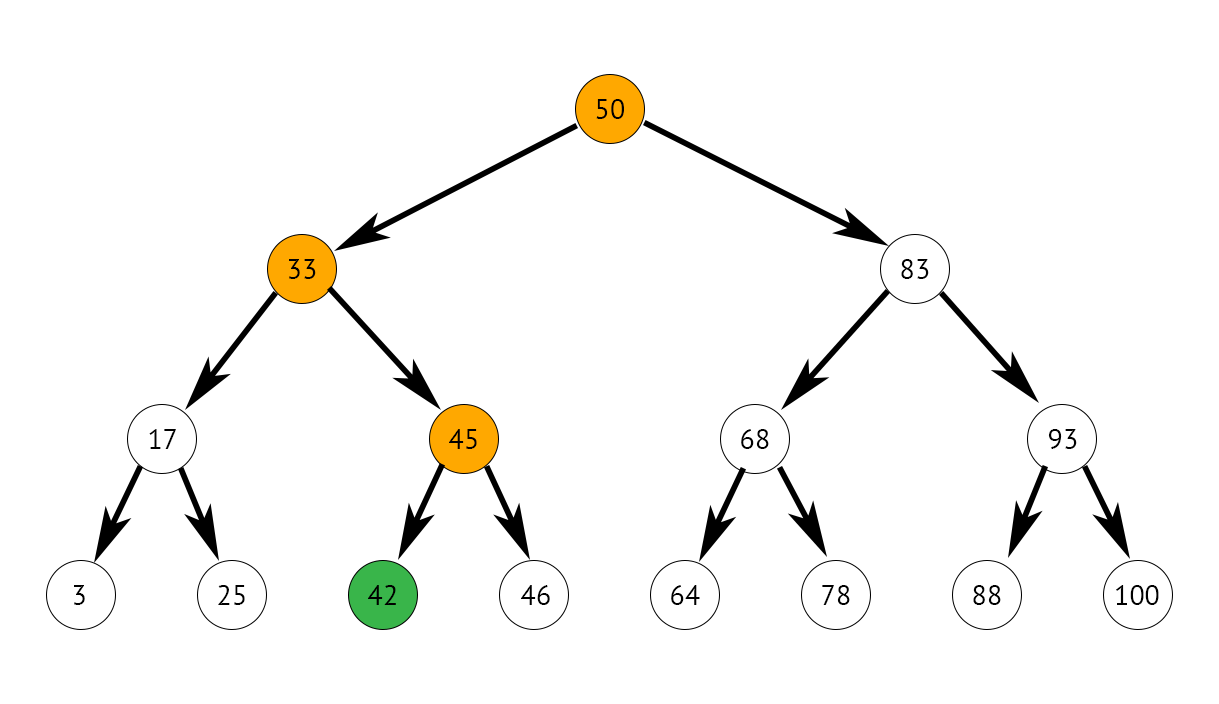
\includegraphics[width=0.9\textwidth]{figures/binary_search_algorithm}
%     \caption[Example of a binary search algorithm run]
%     {\small Example of a binary search algorithm run.
%     The target value is 42.
%     First the root node 50 is compared, but as $42 < 50$ the left subtree is explored.
%     The new root node is 33 and $42 > 30$, so the right subtree is explored.
%     The new root node is 45 and $42 < 45$.
%     The algorithm should search the left subtree, which in this case only consists of one node, with the target value.
%     The search is successful.}
%     \label{fig:binary-search-algorithm}
% \end{figure}

\section{Gaussian Processes}
The Gaussian process \cite{Rasmussen2006} (GP) is a Bayesian non-parametric approach to modelling distributions over functions.
GPs have throughout the years proved themselves useful for solving a wide variety of real-world problems in various fields.
Recent examples of GPs being used are in the field of astronomy to infer intrinsic spectra and stellar radial velocities \cite{Czekala2017} or to infer stellar rotation periods \cite{Angus2017}.
GPs have also been successfully used in the field of Biomedical Engineering to develop a real-time algorithm which scores the risk of intensive care unit admission for ward patients \cite{Alaa2018}.
Finley et al. use GPs to predict forest canopy height \cite{Finley2017}.
In \cite{8082124}, large-scale GPs are used to improve remote sensing image classification and in \cite{Raissi2017} GPs are used to infer linear equation parameters.
In \cite{NIPS2017_6877}, van der Wilk et al. improve the practical aspects for a convolutional structure in GP in order to improve image detection.
In \cite{Stein2017}, Stein conducts a large-scale spatio-temporal data analysis with models based on GPs and in \cite{Dong2017}, Dong et al. perform continuous-time trajectory estimation using GPs.

\subsection{Definition}

Definition \ref{def:gaussian-process} is the formal definition of a GP given by Rasmussen et al. in \cite{Rasmussen2006}.
\begin{definition} \label{def:gaussian-process}
    A Gaussian process is a collection of random variables, any infinite number of which have a joint Gaussian distribution.
\end{definition}

A GP is denoted by the equation
\begin{equation} \label{eq:GP-eq1}
    f(x) \sim \mathcal{GP}(m(x), k(x, x')),
\end{equation}

where the stochastic function $f(\cdot)$ is distributed according to a GP (prior).
The GP is fully specified by
\begin{itemize}
    \item $m(x) = \mathbb{E}[f(x)] = 0$ is the mean function, where the mean function is taken to be zero for notational simplicity \cite{Rasmussen2006};
    \item $k(x, x') = \mathbb{E}[(f(x) - m(x))(f(x') - m(x'))]$ is the covariance function.
    $x$ and $x'$ are two inputs.
\end{itemize}
It can be seen as a probability distribution over functions.
The GP approach is Bayesian as \(f(x) \sim \mathcal{GP}\) encodes a prior belief over the functions.
The covariance function can be expressed in the form of a \textit{kernel}, where different kernels exhibit different characteristics.
A comparison between common kernels is illustrated in Figure \ref{fig:gp-kernels}.
The radial basis function (RBF or SE) kernel and Matérn kernel are given by equations \ref{eq:rbf} and \ref{eq:matern}, respectively.
\begin{align}
k_{\textrm{SE}}(r) &= \sigma^2 \exp{\Big(-\frac{r^2}{2\ell^2}\Big)} \label{eq:rbf} \\
k_{\textrm{Matern}}(r) &= \frac{2^{1-\nu}}{\Gamma(\nu)} \Big(\frac{\sqrt{2\nu}r}{\ell}\Big)^\nu K_\nu\Big(\frac{\sqrt{2\nu}r}{\ell}\Big), \label{eq:matern}
\end{align}
where $\nu$ and $\ell$ are positive parameters, $K_\nu$ is a modified Bessel function and $r = |x-x'|$ \cite{Rasmussen2006}.

If $\nu = 3/2$ in the Matérn kernel, the equation can be simplified to eq. \ref{eq:matern32}.
When $\nu \rightarrow \infty$, the Matérn kernel becomes the RBF \cite{Rasmussen2006}.

\begin{equation} \label{eq:matern32}
    k_{\nu=3/2}(r) = \Big(1+\frac{\sqrt{3}r}{\ell}\Big)\exp{\Big(-\frac{\sqrt{3}r}{\ell}\Big)},
\end{equation}

\begin{figure} [t!]
    \centering
    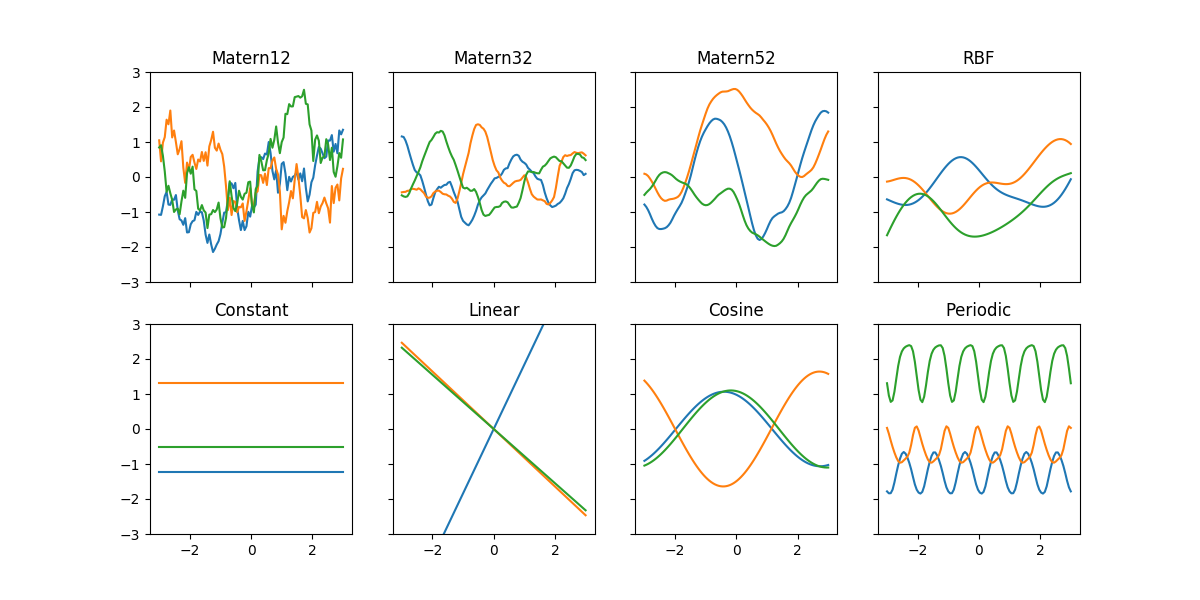
\includegraphics[width=\textwidth]{figures/gp_kernels}
    \caption[Samples from GP priors defined by common covariance functions]
    {\small Samples from GP priors defined by common covariance functions. 
    The functions exhibit different characteristics depending on the choice of kernel and its kernel parameters.}
    \label{fig:gp-kernels}
\end{figure}

Gaussian process regression (GPR) aims at reconstruct the underlying, unknown function without the observation noise $\epsilon$.
The GPR model is given by
\begin{equation}
    y = f(x) + \epsilon,
\end{equation}
where
\[\epsilon \overset{iid}{\sim} \mathcal{N}(0, \sigma_{noise}^2)\]
Here $\epsilon$ represents the noise in each observation, where $\epsilon$ is assumed to be additive independent identically distributed (iid) Gaussian noise.

The posterior of a GP is also a GP \cite{Rasmussen2006}, with a Gaussian predictive distribution given by the posterior GP evaluated at the new point $x_\star$.
The GP prediction (posterior) in a point $x^*$ is defined by the equation
\begin{equation}
    p(y^*|x, y, x^*) \sim \mathcal{N}(\mu_f(x^*), \sigma^2_f(x^*)),
\end{equation}
where
\begin{align}
    \mu_f(x^*) &= K(x^*, x)[K(x, x) + \sigma^2_{noise}I]^{-1}y \\
    \sigma^2_f(x^*) &= K(x^*, x^*) - K(x^*, x)[K(x, x) + \sigma^2_{noise}I]^{-1}K(x,x^*),
\end{align}
where $K(x^*, x), K(x, x)$, and $K(x, x^*)$ each are a covariance (Gram) matrix \cite{Rasmussen2006}.  

\subsection{Related Work} \label{sec:trajectory-aggregation}
GPs have been used with spatio-temporal datasets before to create local trajectory models \cite{Tiger2015-unsupervised-learning,Tiger2015-online-sparse, Tiger2018-gp-motion-pattern}.
In \cite{Tiger2015-unsupervised-learning}, GPs are used to recognise common activities from spatio-temporal datasets.
In \cite{Tiger2015-online-sparse}, sparse GPR is used to perform trajectory modelling.
The methodology conducted can be adapted and implemented in this thesis project.
For example, the equations to aggregate trajectory models can be directly applied in this thesis work.
Tiger et al. specifies two ways to aggregate trajectory models by either Fusion or Combining \cite{Tiger2015-online-sparse}.
The aggregation of trajectory models is useful in order to provide coherent predictions from multiple GPs.
The Combining formula on the predictive mean and variance is given by
\begin{align}
    \mu(x^*) &= \frac{\sum_{j=1}^J N_j \mu_j(x^*) }{\sum_{j=1}^J N_j} \label{eq:combining-mean} \\
    \sigma^2(x^*) &= \frac{\sum_{j=1}^J N_j \big(\sigma^2_j(x^*) + \mu^2_j(x^*)\big)}{\sum_{j=1}^J N_j} - \mu(x^*)^2 \label{eq:combining-var} 
\end{align}
where $N_j$ is the number of trajectories used to train the $j$ trajectory model.
The predictive mean function and predictive variance function are given by $\mu(x^*)$ and $\sigma^2(x^*)$, respectively.

The two approaches are visualised in Figure \ref{fig:aggregation}.
The red Gaussian has mean 0 and variance 0.2, while the blue Gaussian has mean 2 and variance 0.5.
As shown in the figure, the Combining approach creates a Gaussian which captures the variance of all local Gaussians.
\begin{figure} [h!]
    \centering
    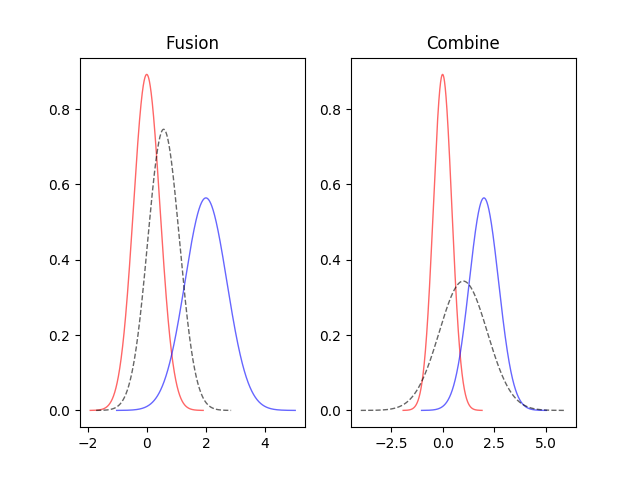
\includegraphics[width=0.7\textwidth]{figures/aggregate_test}
    \caption[Fusion and Combining two Gaussian distributions]
    {\small Fusion and Combining two Gaussian distributions, with $N_1 = N_2 = 1$.
    The red Gaussian distribution has mean 0 and variance 0.2. 
    The blue Gaussian has mean 2 and variance 0.5.}
    \label{fig:aggregation}
\end{figure}


\section{Evaluation Metrics}
Common evaluation metrics when comparing regression models are mean square error (MSE), mean squared logarithmic error (MSLE), and mean absolute error (MAE).

\begin{align}
    MSE(y, \hat{y_i}) &= \frac{1}{n} \sum_{i=1}^{n} (y_i - \hat{y_i})^2 \label{eq:rmse} \\
    MSLE(y, \hat{y_i}) &= \frac{1}{n} \sum_{i=1}^{n} \big( \textrm{ln}(1+y_i) - \textrm{ln}(1+\hat{y_i}) \big)^2 \label{eq:msle} \\
    MAE(y, \hat{y_i}) &= \textrm{median}(|y_1-\hat{y_1}|, \ldots, |y_n-\hat{y_n}|)\label{eq:mae}
\end{align}

Typically, the root of the MSE (RMSE) is used as a metric
\begin{equation}
    RMSE(y, \hat{y_i}) = \sqrt{MSE(y, \hat{y_i})}
\end{equation}
RMSE is susceptible to outliers affecting the performance of the metric, as it causes a large variability of the errors \cite{Willmott2005}.
MSLE partly solves the variability of large errors by applying the natural logarithm to the targets $y_i$ and $\hat{y_i}$, respectively.
MAE is resistant to outliers, as it only looks at the median of all errors.
MAE is praised in \cite{Willmott2005} by Willmott et al., while Chai et al. defend the use of RMSE in \cite{Chai2014}.
For example, RMSE is shown in \cite{Chai2014} to be a useful metric if the errors follow a Gaussian distribution.

\section{GPflow}
GPflow\footnote{https://gpflow.readthedocs.io/en/latest/index.html} \cite{GPflow2017} is a GP framework for the Python\footnote{https://www.python.org/} programming language, using TensorFlow\footnote{https://www.tensorflow.org/}.
It is an open-source software which has its origins from the contributors of GPy\footnote{https://sheffieldml.github.io/GPy/}, another famous framework for implementing GPs in Python.
As GPflow is built upon TensorFlow, it achieves better performance when using GPUs for processing \cite{GPflow2017}.
The GPy background and TensorFlow foundation contribute with quality of life features which facilitates easier development, such as automatic differentiation. 
Building GPflow on top of TensorFlow also allows the benefits of using TensorFlow methods for calculations, e.g., most gradient computations are handled by TensorFlow.
All models in this thesis project are implemented using the GPflow framework.

% \section{Finite-State Machines}
% Finite-state machines (FSM) are well-defined mathematical models which can have numerous representations.
% The formal notation used here are from the book "Automata and Computability" by Kozen \cite{Kozen1997}.
% An FSM is defined as a set of states with potentially multiple transitions between each state.
% The FSM can only be in one given state at any time.

% Formally an FSM is given by the structure
% \[M = (Q, \Sigma, \delta, s, F),\]
% where
% \begin{itemize}
%     \item Q is a finite set of states.
%     \item $\Sigma$ is the input alphabet of the FSM.
%     \item $\delta : Q \times \Sigma \rightarrow Q$ is the transition function for the FSM.
%     It can intuitively be seen as the function which tells the FSM which state to transition to in response to an input.
%     For example, if M is in state $q$ and receives input $x$ it should move to state $\delta(q, x)$.
%     \item $s \in Q$ is the start state.
%     \item $F \subset Q$; where the elements of $F$ are the final states of the FSM.
% \end{itemize}

% An FSM can be modelled with various representations \cite{Kozen1997}, e.g, in tabular form, as a transition diagram or as a regular expression.

\section{Exploratory Data Analysis}
Exploratory Data Analysis (EDA) is a broad concept comprising various techniques for exploring and analysing data \cite{Anselin1999, Gelman2003, Hoaglin2003, Tukey1977, Velleman1981}.
Early popular techniques include \emph{box plots} and \emph{stem-and-leaf} displays.
A stem-and-leaf plot takes numbers and splits them into two groups.
The first group contains the leading digit(s) and the second group contains the trailing digit(s).
Figure \ref{fig:stem-leaf-plot} is an example of a stem-and-leaf plot with one leading and one trailing digit.
The grouping helps when sorting batches of data and visualising important features, without losing the information of any single data point used \cite{Velleman1981}.

\begin{figure} [h!]
    \centering
    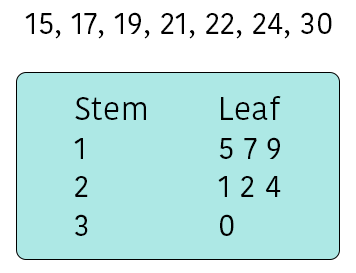
\includegraphics[width=0.33\textwidth]{figures/stem-leaf-plot}
    \caption[Example of a stem-and-leaf plot]
    {\small Example of a stem-and-leaf plot. The numbers above the plot is the input.
    The first digit of the number is the \emph{stem}, the following digits are the \emph{leafs}.}
    \label{fig:stem-leaf-plot}
\end{figure}

EDA can be seen as the application of tools and statistical methods to analyse data in a meaningful way, e.g., it can be applied to the detection of outliers, smoothing the data, or performing a variance analysis \cite{Anselin1999, Hoaglin2003, Tukey1977, Velleman1981}.
EDA can also reveal subtle practical problems with the chosen model that can easily be missed when performing statistical analysis of the model \cite{Gelman2003}.

In \cite{Tukey1977}, Tukey describes how EDA can be used to answer research questions such as "What is the age distribution for the Vietnamese population?" and "Are there differences in
the annual household per capita expenditures between the rural and urban populations in Vietnam?".
Tukey uses plots to compare different groups and estimators, such as the sample mean estimator, or the \emph{winsorised} mean, to quantify the difference.
The winsorised mean handles the case where tails of a distribution dominates the value space.  
This causes the sample mean estimator to poorly reflect on the "typical" data point, as it is skewed by the small tail population \cite{Tukey1977}.

In \cite{Velleman1981}, Velleman et al. present different EDA techniques and highlights four key areas of EDA: displays (plots), residuals, re-expressions and resistance.
Residuals are what remain after data analysis is performed.
Residuals can, for example, be what remains after fitting data to a model (the error of the fit) \cite{Velleman1981}.
Re-expression is the notion of applying mathematical functions to the data.
Re-expressing the data can help with the data analysis \cite{Hoaglin2003, Velleman1981}.
Examples of mathematical functions that can be applied are: logarithm, square root, reciprocal square function or generally raising the data to some power $p$.
Resistance is the concept that outliers should not disproportionately affect the data analysis \cite{Hoaglin2003, Velleman1981}.
For example, the winsorised mean estimator is less sensitive to localised misbehaviour than the sample mean estimator \cite{Tukey1977}.

Smoothing data is important for many different applications \cite{Bradley1997, Pang2002, Quinlan1992, Velleman1981}.
This can, for example, be done by applying \emph{running median smoothers}.
The running median smoothers go through all the data points in sequence and calculate only the median for the $n$ closest values near each point \cite{Velleman1981}.
Another approach is the \emph{running weighted average} \cite{Velleman1981}.
Instead of taking the median of the $n$ values, the average is calculated.
The average can also be weighted with different functions, like hanning smoothing \cite{Velleman1981}.
The hanning smoothing for three data points is shown in Eq. \ref{eq:hanning}.
It is worth noting that a single outlier heavily affects the hanning smoothing and that in practice it is common to first apply a running median smoothing to remove outliers \cite{Velleman1981}.

\begin{equation}
    \hat y_t = \frac{1}{4} y_{t-1} + \frac{1}{2} y_t + \frac{1}{4} y_{t + 1} 
    \label{eq:hanning}
\end{equation}